\begin{scanpage}{0116}{99}
\noindent\begin{minipage}[t]{.48\linewidth}\vspace{0pt}\centering
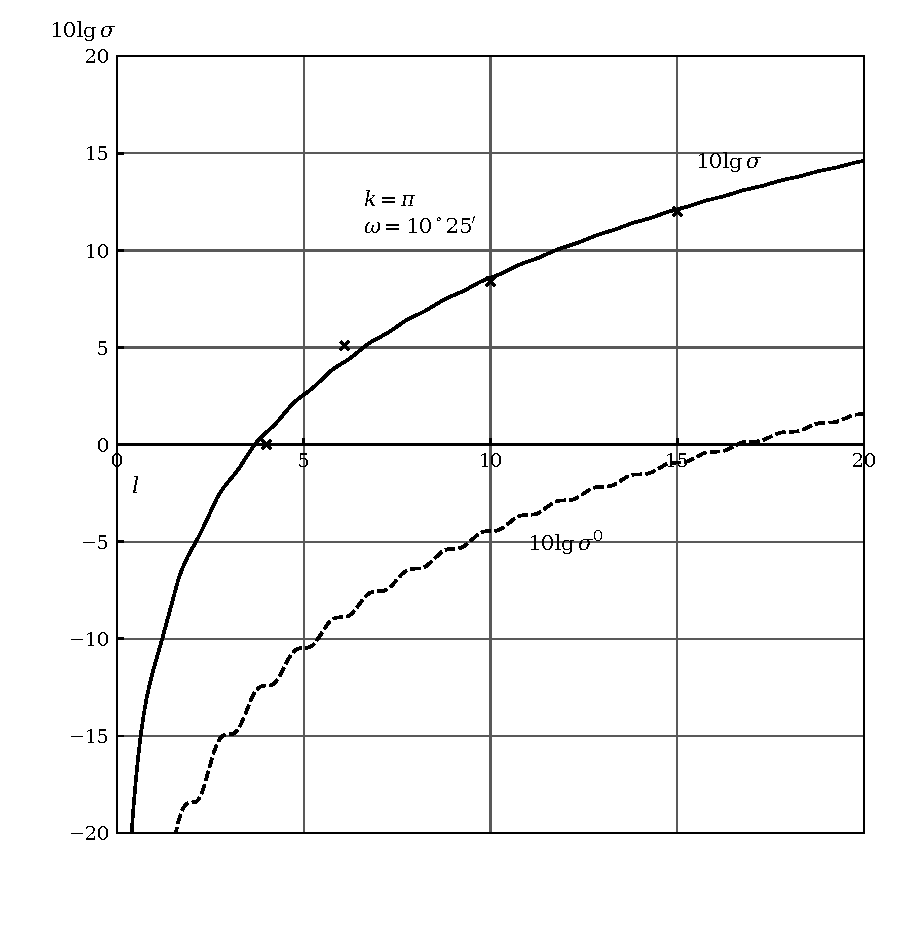
\includegraphics[width=.9\linewidth]{images/recreated/b-0116-fig31.pdf}

\raggedright Figure 31. The effective scattering area of a finite cone as a function of its length. The function $\sigma$ (the continuous line) was calculated on the basis of equation (17.06) which considers the nonuniform part of the current in the vicinity of the circular discontinuity. The function $\sigma^0$ (the dashed line) corresponds to the physical optics approach.
\end{minipage}\hfill\begin{minipage}[t]{.48\linewidth}\vspace{0pt}
with its deformation into a disk $(\omega\to90^\circ)$. The discrepancy between our curve and the physical optics approach here reaches almost 30 dB when $\omega=2^\circ$.

Expression (17.08) obtained by us also allows one, in contrast to the physical optics approach (17.09), to evaluate the role of the shape of the shadowed part of the body and shows that the reflected signal will be larger, the closer this shape is to a funnel-shaped form $(\Omega\approx\pi-\omega)$. Thus, for example, in the case $\omega=10^\circ$, $kl=10\pi$ $(k=\pi)$ the signal reflected by the cone may exceed by 15 dB the value corresponding to physical optics (see Figure 33) if $\Omega\approx170^\circ$.
\end{minipage}\par\medskip

Let us note that our Expression (17.13) is equivalent to the expression presented in the above-mentioned papers [41, 44]. However, the latter expression is applicable only for sharply pointed cones, whereas we have, in addition to (17.13), Equation (17.08) which is suitable for cones with any aperture angle $\omega$ $(0\leq\omega\leq\frac\pi2)$.

The calculation method discussed may be generalized in the case of asymmetric irradiation of the cone. However, with asymmetric irradiation, generally speaking, it is necessary to take into account the nonuniform part of the current caused by the point of the cone.

In concluding this section, let us calculate the effective scattering area for a body which is formed by rotation around the
\end{scanpage}
